%-------------------------------------------------------------------------------
\FloatBarrier\section{Solutions}
%-------------------------------------------------------------------------------



%-------------------------------------------------------------------------------
\subsection{Quiz}
%-------------------------------------------------------------------------------

\begin{boenumerate}

\item \textbf{False}, this depends on the share of low productivity workers.

\item \textbf{False}, it is zero for the last transition.

\item \textbf{False}, it only allows to interpret the coefficient as an average growth rate of wages with schooling. This is only true in the compensating-differences model by construction.

\item \textbf{False}, this depends on whether individuals are forward-looking or not.

\item  \textbf{Ambiguous}, this depends on the outcome under investigation. In particular for some social outcomes, the effect of noncognitive skills is more pronounced.

\item  \textbf{False}, the extended model does a much better job at explaining the observed choice patterns. In particular, the persistence in choices is better captured. For example, the extended version includes mobility costs that discourage switching between occupations.

\item \textbf{True}, the test and reject the hypothesis that individuals do not.

\item \textbf{False}, it is initial unobserved heterogeneity that accounts for most of the observed inequality in expected total lifetime utility.

\item \textbf{True}, this is their conclusion.

\item \textbf{False}, their finding is the exact opposite. Instead, it is rich countries where wages increases stantially more over the life cycle.

\item \textbf{False}, they restrict their analysis to full time workers throughout.

\item \textbf{False}, instead they point to human capital and search as reasonable explanations for the observed patterns. Long-term contracts can explain flatter
experience-wage profiles in poor countries in two scenarios. The first scenario is that wages are more front-loaded in poor countries. In this case we would expect day laborers in poor countries to have steeper profiles than the rest of the workforce. The second scenario is that wages are more back-loaded in rich countries. In this case, we would expect day laborers in rich countries to have flatter profiles. We find no evidence of either of these scenarios.

\item \textbf{True}, they only rule out long-term contracts.

\item \textbf{False}, while the withing-sample model fit is similar the predictions of the models differ considerably. For example, the static model does indicate that all individuals will work in a white collar occupation. The dynamic model points towards an equal allocation across occupations.

\item \textbf{False}, they document a considerable effect on High School and College graduation rate instead. Individuals induced to pursue increased schooling due to the sidy do end up working in the same occupations in the end and thus there is no real effect on their lifetime utility.

\item \textbf{False}, at least the point estimates indicate a negative effect for individuals with a large dislike for treatment participation.

\item \textbf{False}, they present models and return concept that allow to distinguish between ex ante and ex post return to schooling.

\end{boenumerate}
%-------------------------------------------------------------------------------
\FloatBarrier\subsection{Introduction}
%-------------------------------------------------------------------------------

\begin{boenumerate}
\item Both models are designed as to explain why individuals invest in their human capital. The key difference is in the productivity effect of human capital. In \cite{Ben-Porath.1967} human capital does increase productivity, while in \cite{Spence.1973} it does not. Numerous features are missing from both models. Among those discussed in class are a lack of distinction between general and specific training, uncertainty, and borrowing constraints.

\item From the graphs it follows that:

\begin{align*}
w_L(y) = w_H(z) = \begin{cases}
1 & \text{if}\quad y < y^*  \\
2  & \text{if}\quad y \geq y^*  \\
\end{cases}
\end{align*}

and

\begin{align*}
c_L(y) & = y           \\
c_H(y) & = \tfrac{2}{3}\, y
\end{align*}

\item Individuals receive a wage for working but also incur a cost of investing in human capital.

\begin{align*}
s_j(y) = \begin{cases}
w_L - c_j(y) & \text{if}\quad y < y^*  \\
w_H - c_j(y) & \text{if}\quad y \geq y^*  \\
\end{cases}
\end{align*}

For the parametrization in this particular case:

\begin{align*}
s_L(y) = \begin{cases}
1 - y & \text{if}\quad y < y^*  \\
2 - y & \text{if}\quad y \geq y^*  \\
\end{cases}
\end{align*}

\begin{align*}
s_H(y) = \begin{cases}
1 - \tfrac{2}{3}\,y & \text{if}\quad y < y^*  \\
2 - \tfrac{2}{3}\,y & \text{if}\quad y \geq y^*  \\
\end{cases}
\end{align*}


Figure \ref{Surplus} shows the visual presentation.

\begin{figure}[h]\centering
\caption{Surplus}\label{Surplus}
\scalebox{0.35}{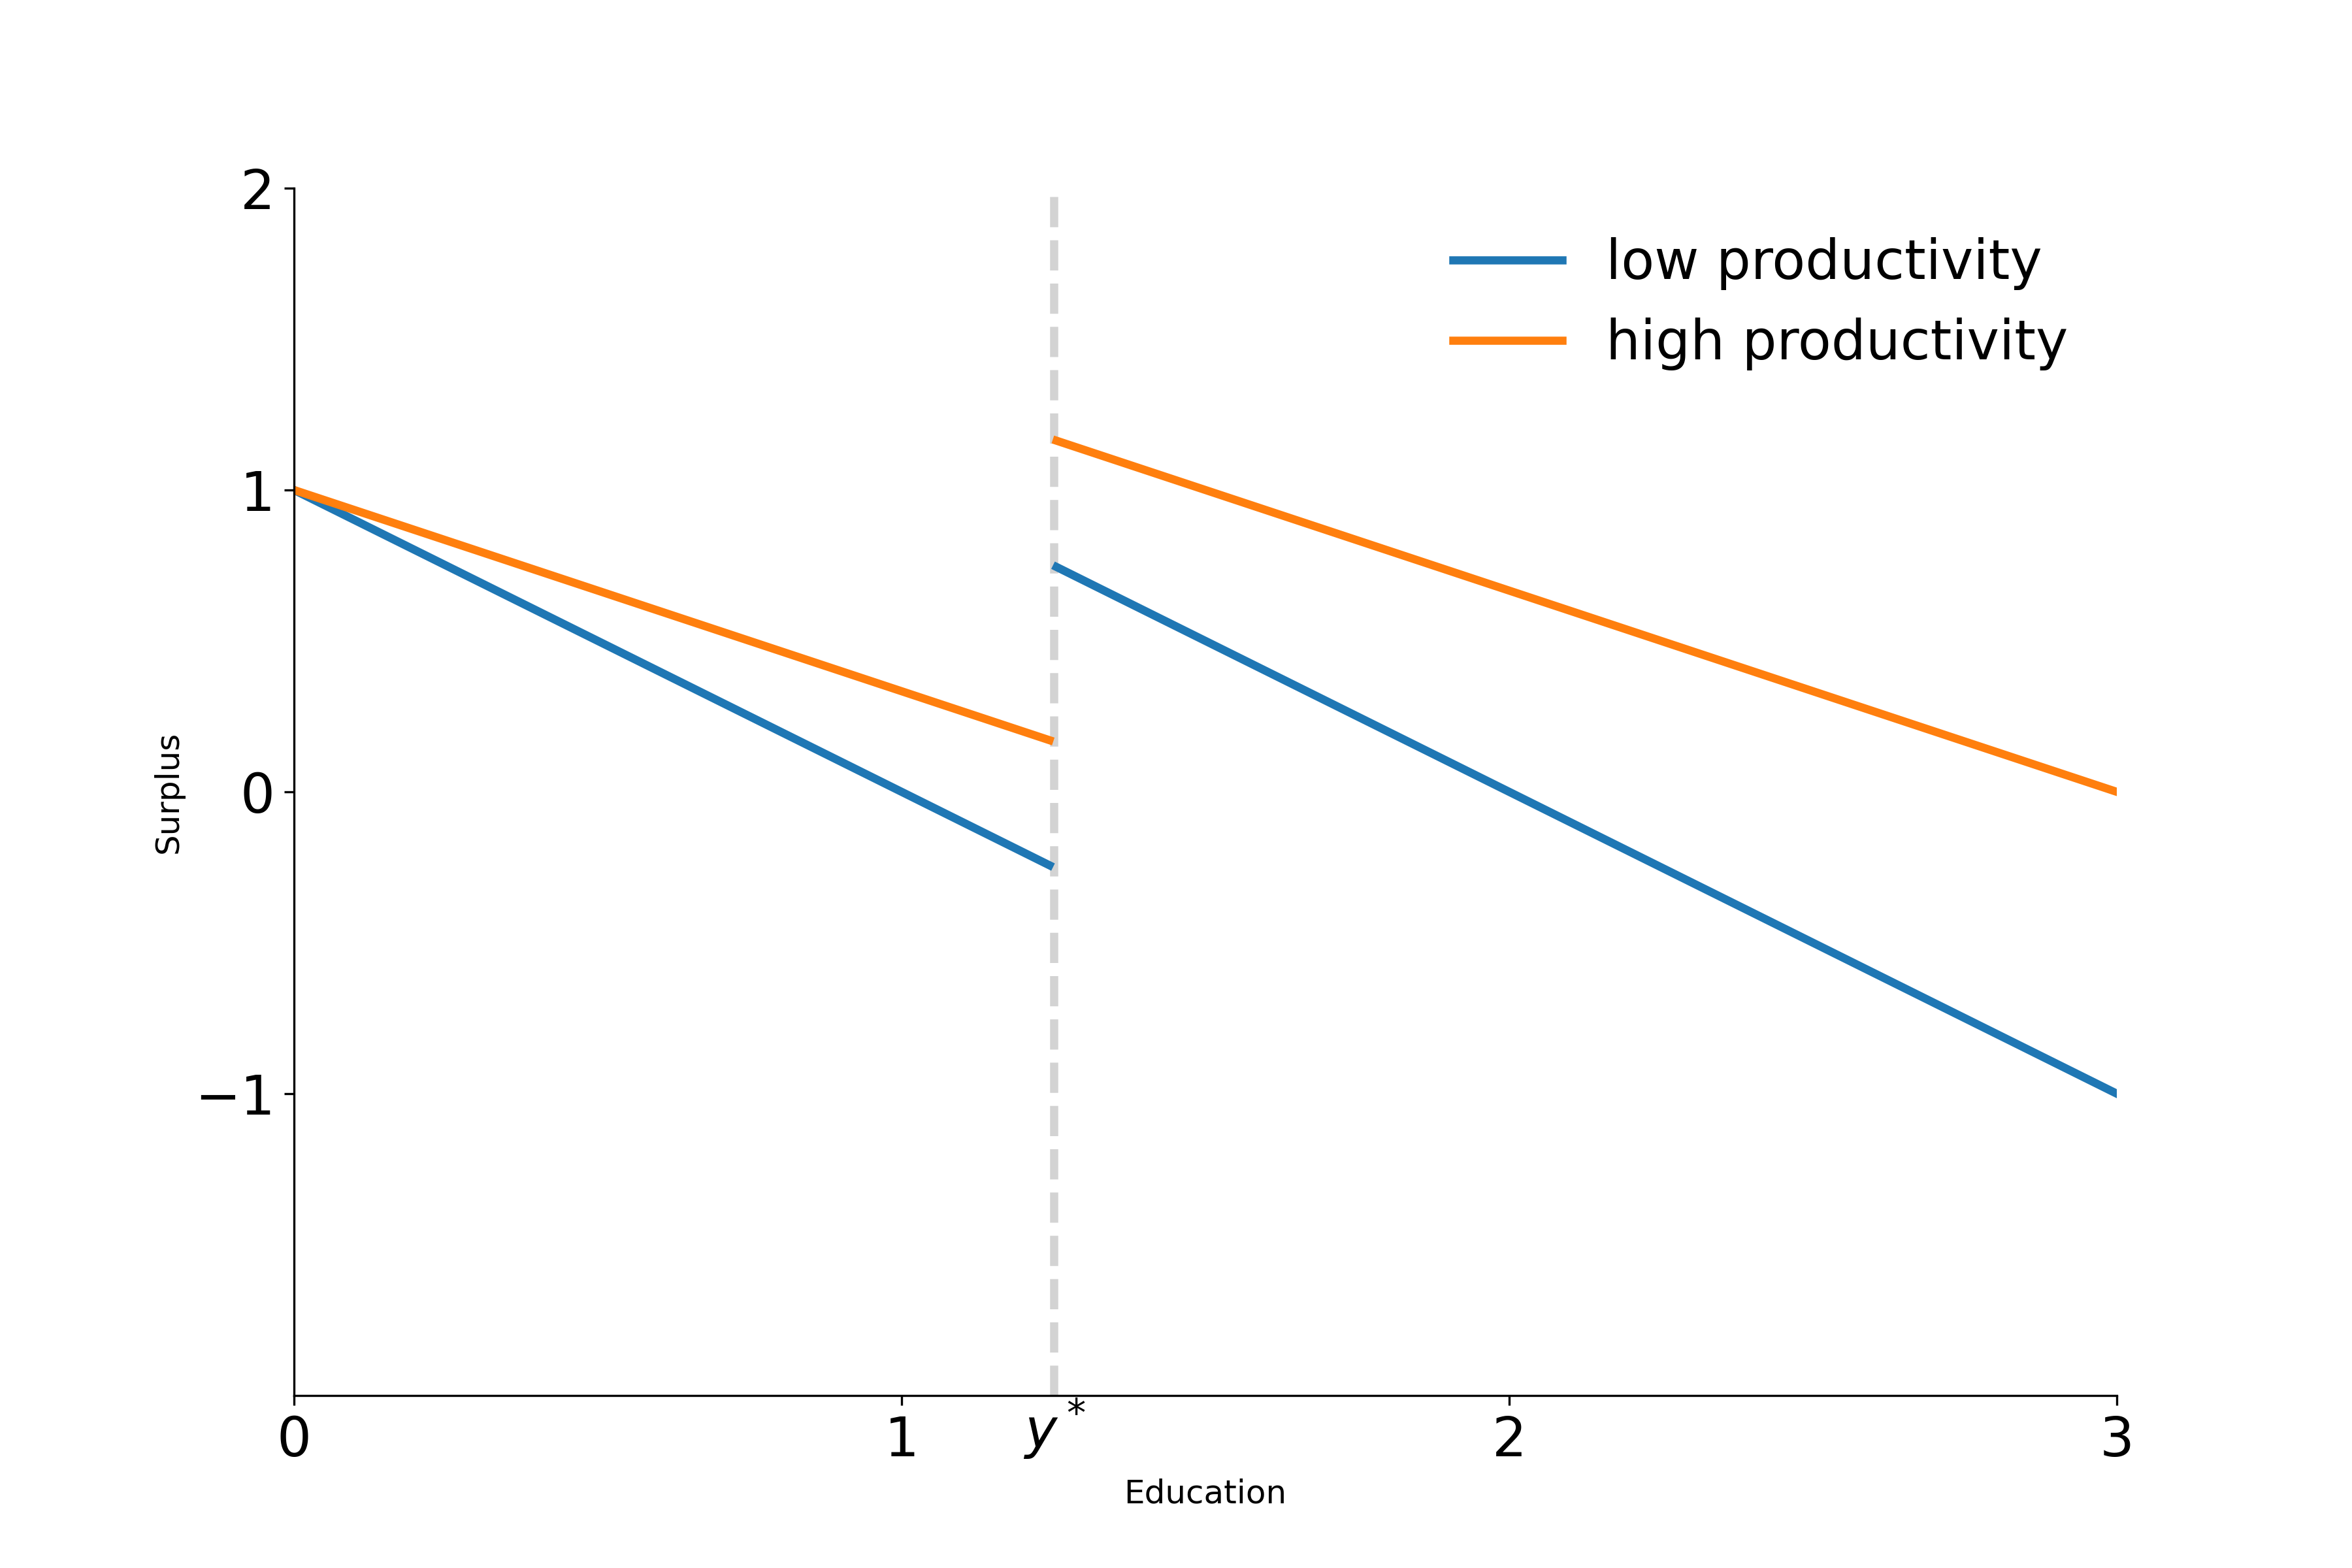
\includegraphics{fig-introduction-spence-surplus}}
\end{figure}

\item The separating level of schooling needs to be high enough that low productivity individuals do not pursue any schooling and still low enough so that high productivity individuals find it fruitful to do so. So, these two equations have to be fulfilled at the same time.

\begin{align*}\begin{array}{lll}
1  > 2 - y^*        &\xrightarrow &  y^* > 1 \\
1  < 2 - \frac{2}{3}\, y^* &\xrightarrow &  y^* < \frac{3}{2}
\end{array}
\end{align*}

And thus the employer's beliefs are confirmed if $1 < y^* < \tfrac{3}{2}$.

\item In the absence of signaling, the wage is simply the unconditional expected marginal product and there is no reason to invest in one's human capital $(y = 0)$.

\begin{align*}
\bar{w} = q_L \times 1 + (1 - q_L) \times 2
\end{align*}

\item Figure \ref{Market Structure} shows the market structure.

\begin{figure}[h]\centering
\caption{Market Structure}\label{Market Structure}
\scalebox{0.35}{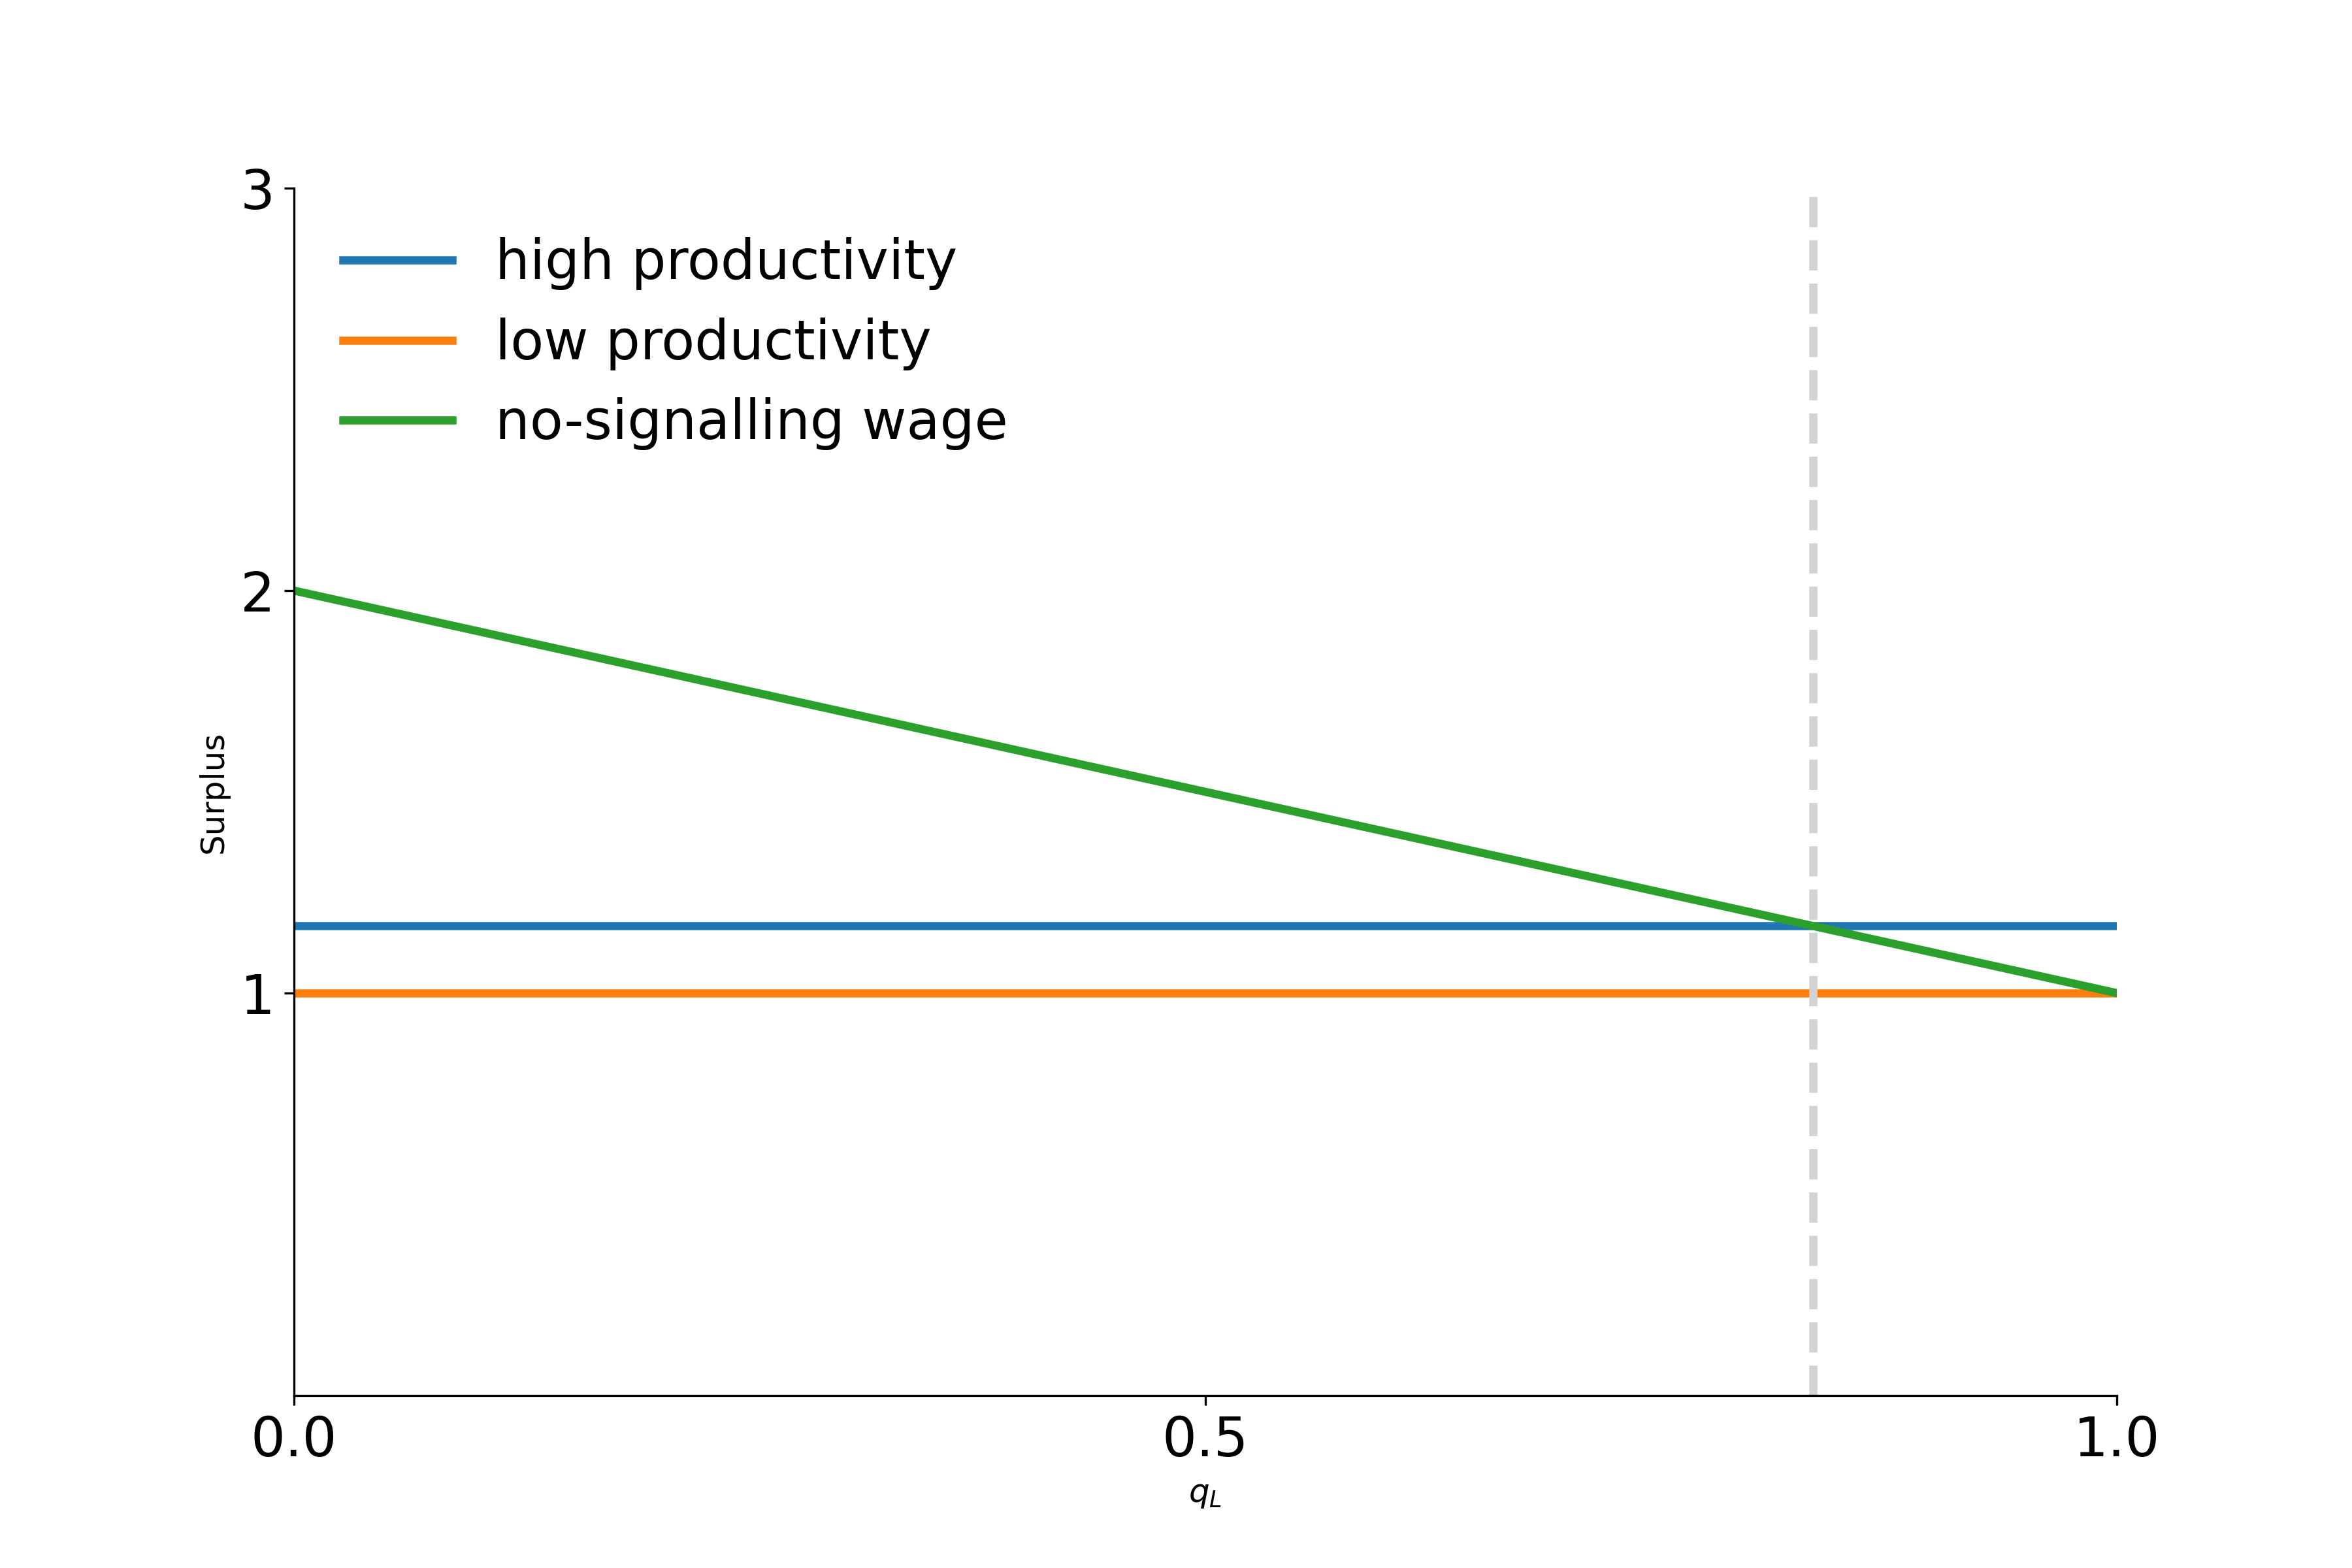
\includegraphics{fig-introduction-spence-market-structure}}
\end{figure}

\item The high productivity individuals' preferences depend on the share of the low productivity individuals. The wage, which corresponds to the surplus as $y = 0$, is easily computed.

\begin{align*}
s_h = w_h = 2 - q_L.
\end{align*}

The surplus in the case of signaling and $y^* = \frac{5}{4}$ is computed as:

\begin{align*}
s_h & = 2 - \frac{2}{3}\frac{5}{4} \\
    & = 2 - \frac{10}{12} = \frac{7}{6}.
\end{align*}

The surplus for the high productivity individuals is equal in both scenarios at $q_L = \frac{5}{6}$

\end{boenumerate}

%-------------------------------------------------------------------------------
\FloatBarrier\subsection{Static model of educational choice}
%-------------------------------------------------------------------------------

\begin{boenumerate}
\item Please see below for the key equations of the model.
\begin{align*}\begin{array}{l@{\qquad}l}
        \text{Potential Outcomes} &\text{Observed Outcome}\\
        Y_1 = \mu_1(X) + U_1      &  Y = D Y_1 + (1 - D)Y_0 \\
        Y_0 = \mu_0(X) + U_0      &\\
        & \\
        \text{Choice} & \\
        D = \mathrm{I}[\mu_D(X, Z) - V > 0] & \\
    \end{array}
\end{align*}

\item Given the notation above, the definition of the conventional average effects of treatment is straightforward.

\begin{align*}
    B^{ATE} & = E[Y_1 - Y_0 ]\\
    B^{TT} & = E[Y_1 - Y_0 \mid D = 1]\\
    B^{TUT} & = E[Y_1 - Y_0 \mid D = 0]\\
\end{align*}

Their policy-relevance is limited, as they correspond to extreme policy alternatives. For example a stylized version of the Affordable Care Act, where health insurance coverage was universal after the implementation of the reform. As a considerable share of Americans was already covered before, this corresponds to the $B^{TT}$. A focus on average affect might mask considerable heterogeneity in benefits.

\item The concept of essential heterogeneity describes the idea that individuals select their treatment status based on unobservable gains from treatment even after conditioning on unobservables. More formally,

\begin{align*}
    Y_1 - Y_0 \notindep D\quad \mid X = x.
\end{align*}

In the presence of essential heterogeneity, the conventional average treatment effects differ. They coincide in the absence of essential heterogeneity. Thus the figure is a simple replication from the lecture slides.

\item The marginal benefit is the average effect of treatment for individuals at different quantiles of the first-stage unobservable $V$. More formally,

\begin{align*}
    B^{MTE}(x, u_D) = E [Y_1 - Y_0 \mid X = x,  U_D = u_D].
\end{align*}

Figure \ref{Marginal Benefit of Treatment} shows the marginal benefit of treatment in the presence and absence of essential heterogeneity.

\begin{figure}[h]\centering
\caption{Marginal Benefit of Treatment}\label{Marginal Benefit of Treatment}
\scalebox{0.35}{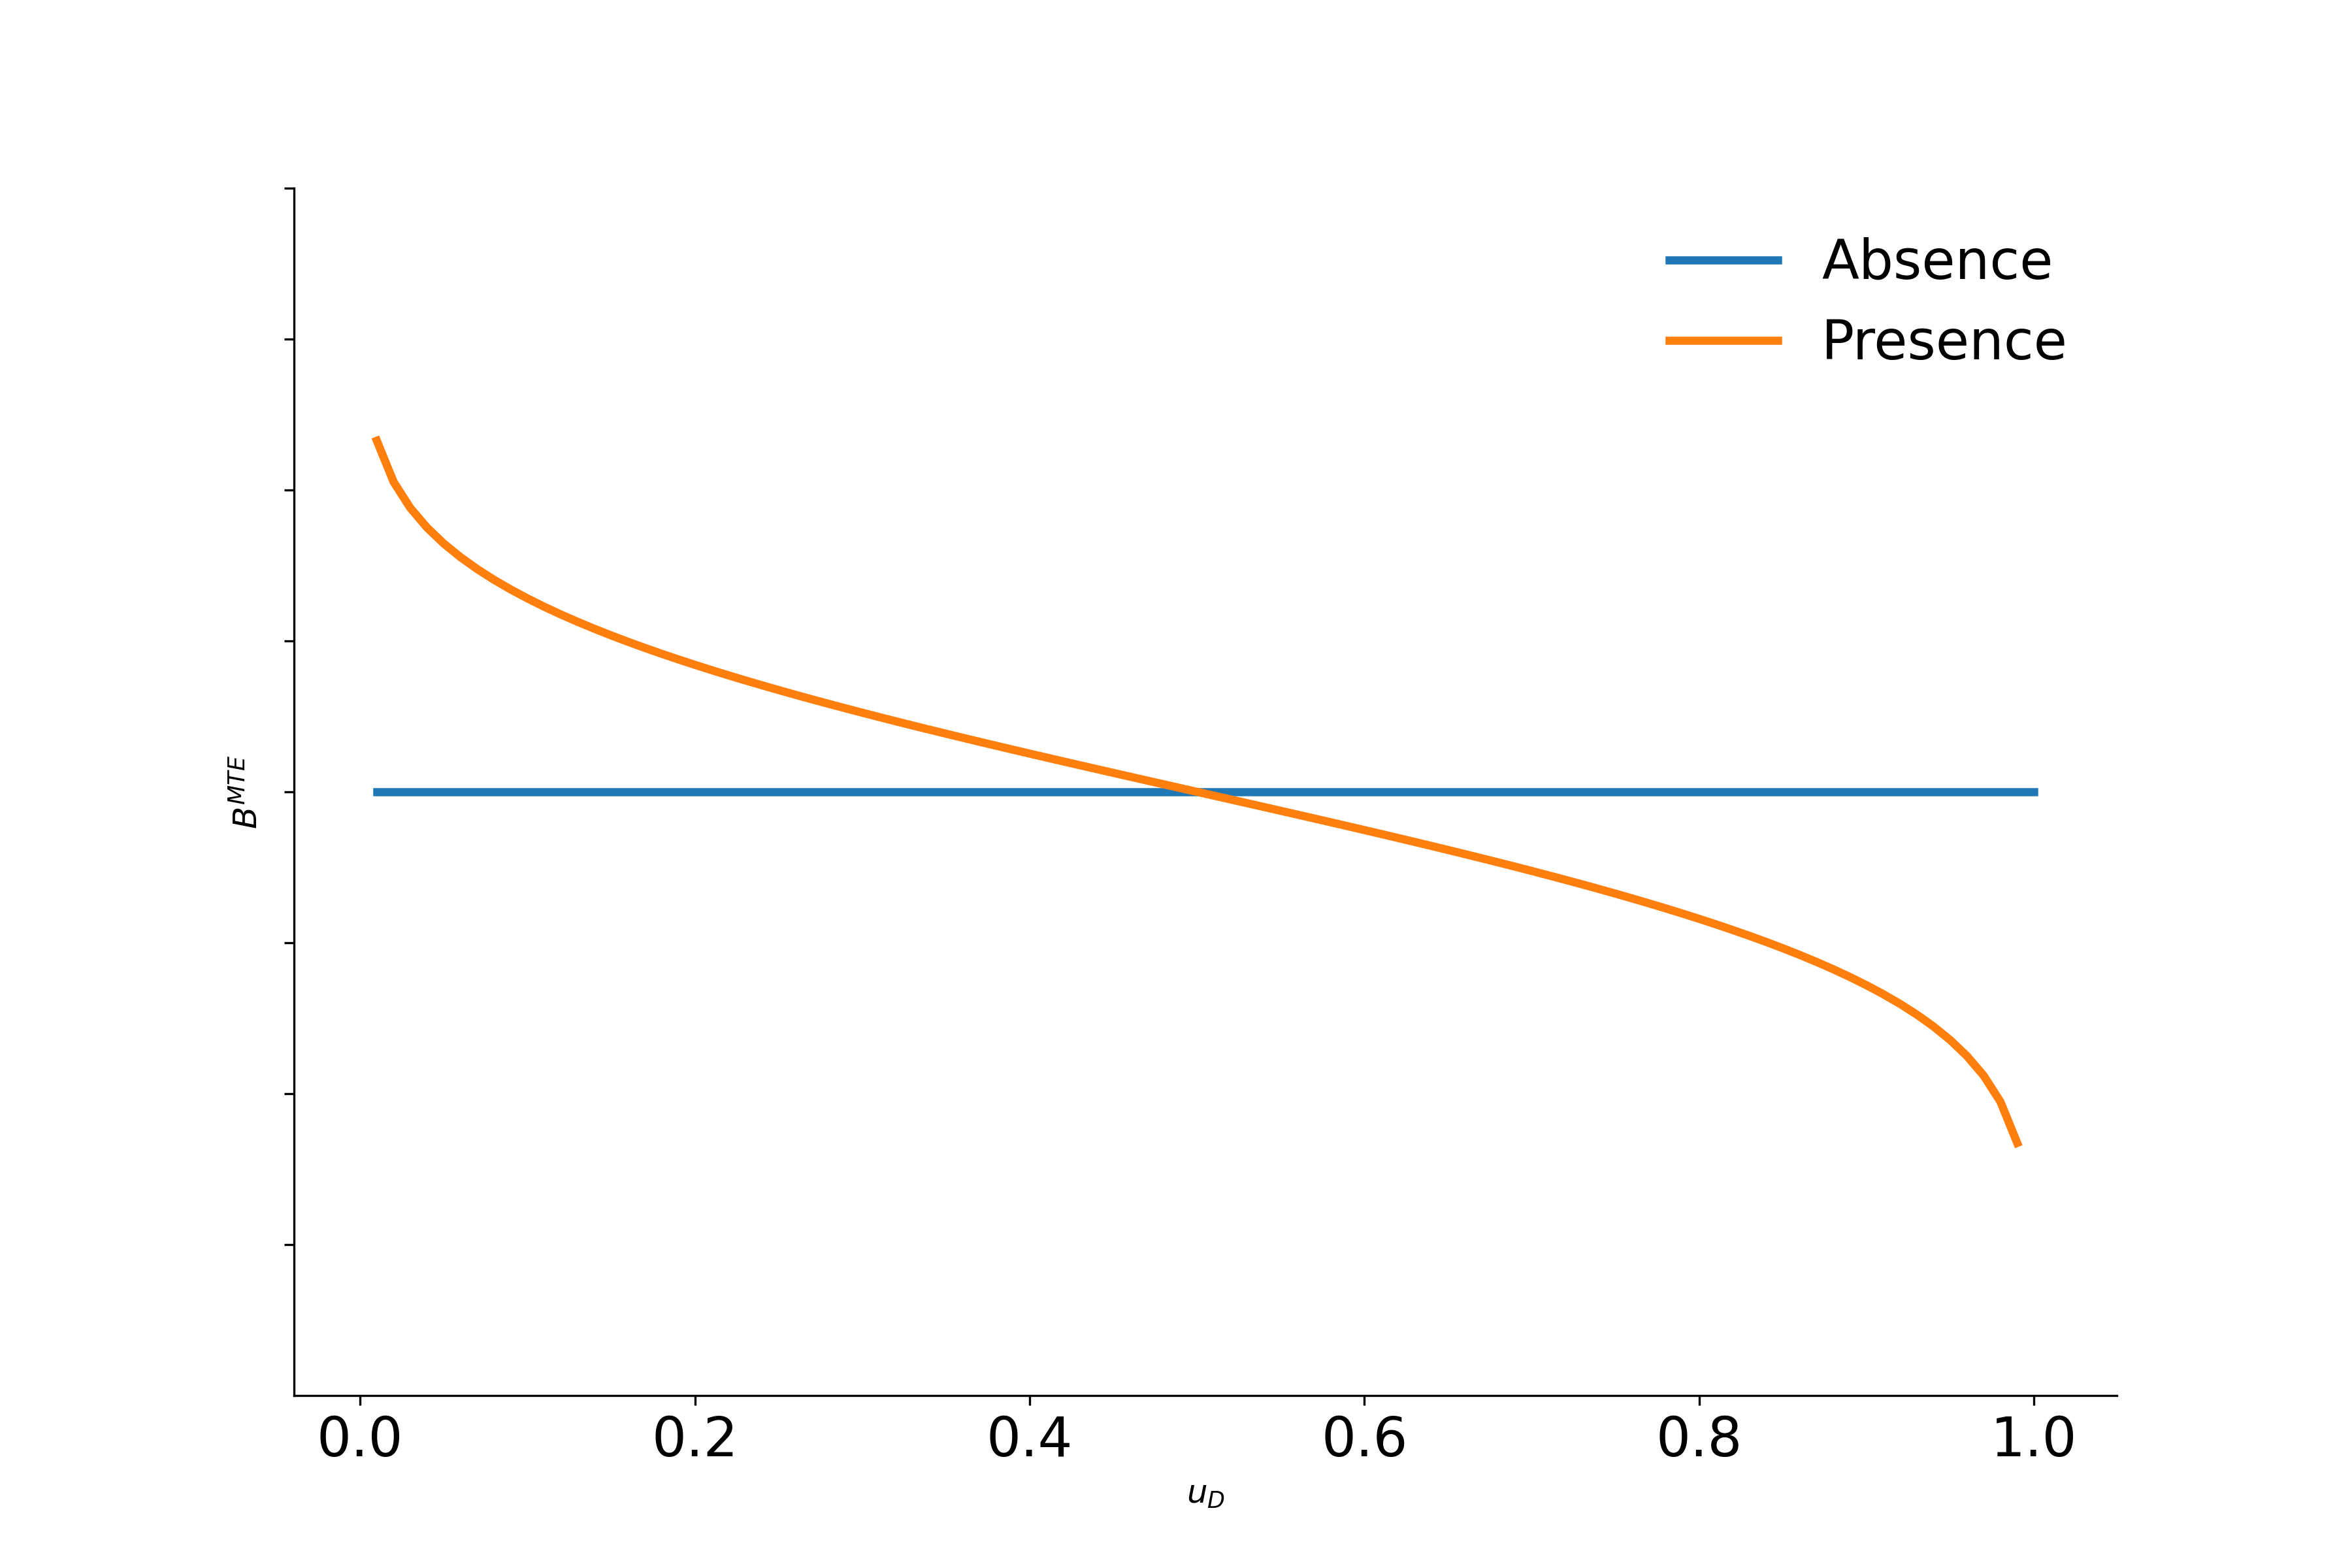
\includegraphics{fig-static-model-marginal-benefit}}
\end{figure}

\item \cite{Carneiro.2011} document considerable heterogeneity in the returns to a college education. They range from $40\%$ to $-20\%$ evaluated at the mean values of the sample's observables.

\item The static model does not account for the dynamic nature of educational choices, where uncertainty reveals information about its benefits and cost throughout one's educational career.
\end{boenumerate}

\begin{boenumerate}
\item The individual effect of treatment $B$ is defined as the difference in potential outcomes $Y_1 - Y_0$. The unobservable $U$ is the only source of heterogeneity in the model. Given its distribution and the selection equation, about 50\% of individuals will select into treatment. However, only about 25\% have a positive benefit of treatment.

\item The conventional average treatment effects are defined below.
%
\begin{align*}
    B^{ATE} & = E[Y_1 - Y_0 ]\\
    B^{TT}  & = E[Y_1 - Y_0 \mid D = 1]\\
    B^{TUT} & = E[Y_1 - Y_0 \mid D = 0]
\end{align*}
%
Their policy-relevance is limited, as they correspond to extreme policy alternatives. For example a stylized version of the Affordable Care Act, where health insurance coverage was universal after the implementation of the reform. As a considerable share of Americans was already covered before, this corresponds to the $B^{TT}$. A focus on average effects might mask considerable heterogeneity in benefits.

Figure \ref{Distribution of benefits} shows the distribution of benefits. All individuals with a benefit above -0.25 select into treatment because it still holds that $0.50 > U$.

\begin{figure}[htp]\centering
\caption{Distribution of benefits}\label{Distribution of benefits}
\scalebox{0.5}{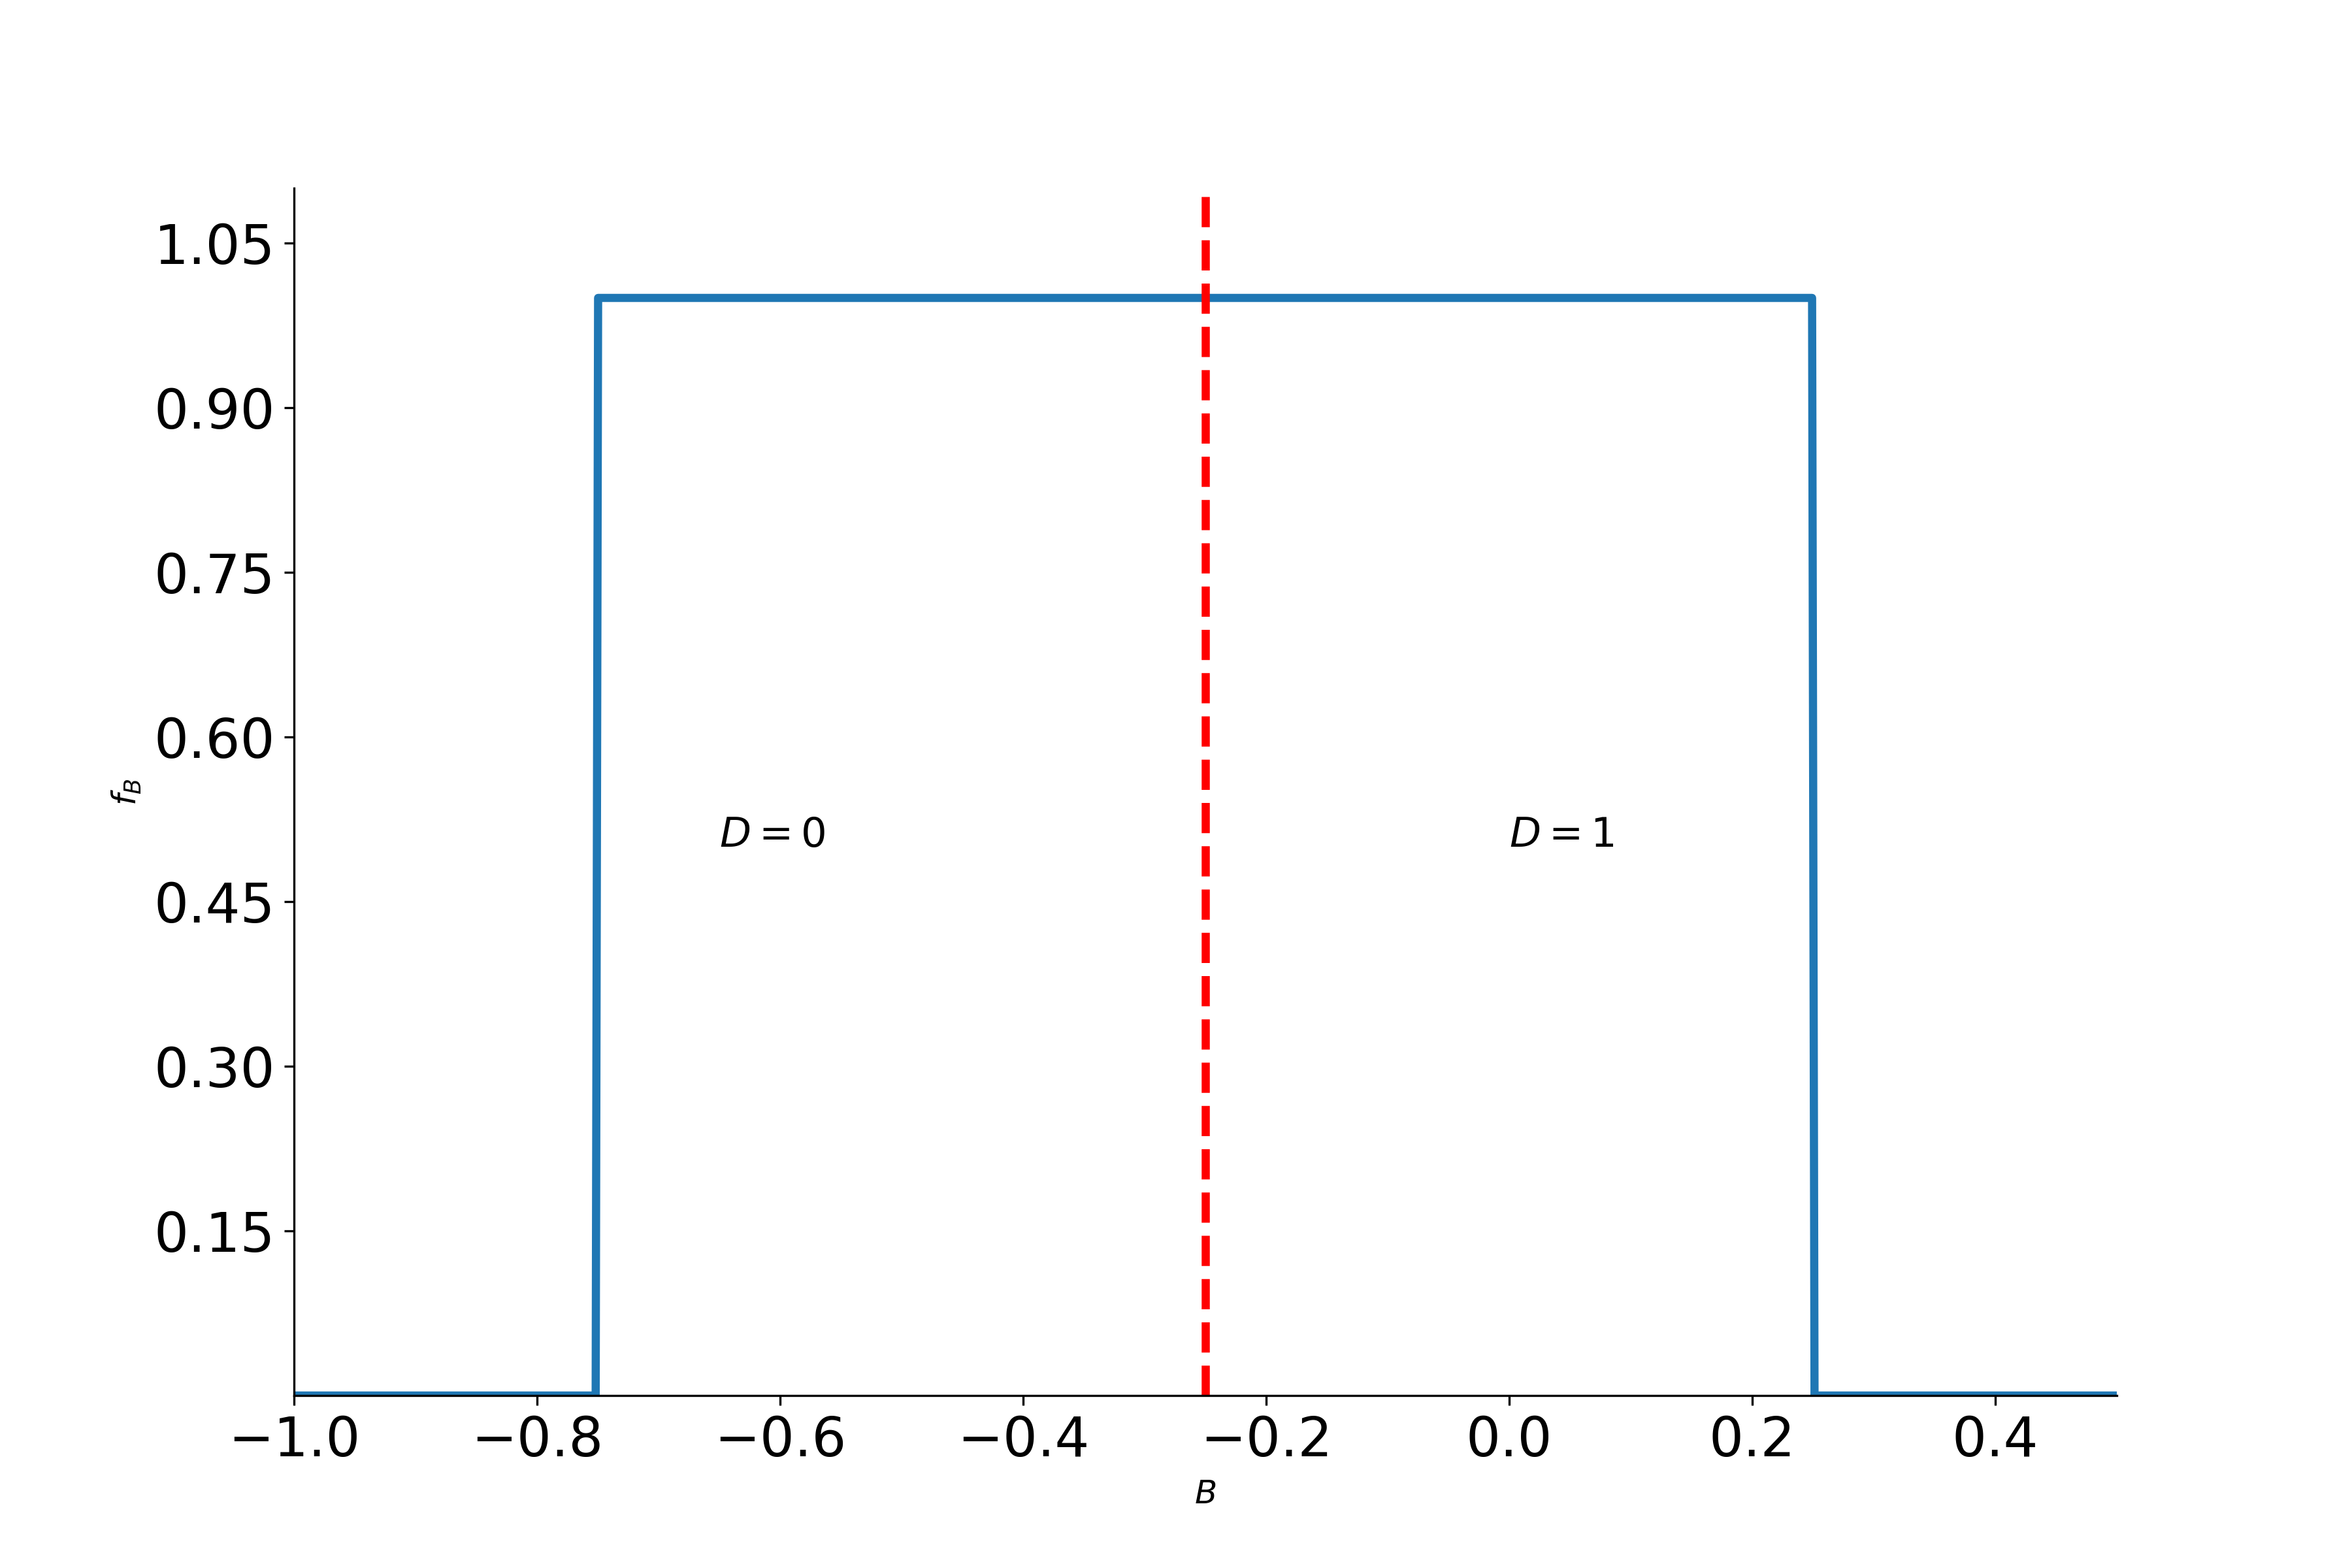
\includegraphics{fig-static-model-distribution-benefits}}
\end{figure}

The conventional effects of treatment are calculated as:
%
\begin{align*}
    B^{ATE} & = -0.25 \\
    B^{TT}  & =  0.00\\
    B^{TUT} & = -0.50
\end{align*}

\item The concept of essential heterogeneity describes the idea that individuals select their treatment status based on unobservable gains from treatment even after conditioning on unobservables. More formally,

\begin{align*}
    Y_1 - Y_0 \notindep D\quad \mid X = x.
\end{align*}

The parameterized model does exhibit essential heterogeneity as individuals with the highest dislike to select into treatment $U$ have the least to gain.

\item The marginal benefit is the average effect of treatment for individuals at different quantiles of the first-stage unobservable $V$. More formally,

\begin{align*}
    B^{MTE}(u_D) = E [Y_1 - Y_0 \mid U_D = u_D].
\end{align*}

Figure \ref{Marginal benefit of treatment} shows the marginal benefit of treatment for the parameterized model.

\begin{figure}[htp]\centering
\caption{Marginal benefit of treatment}\label{Marginal benefit of treatment}
\scalebox{0.50}{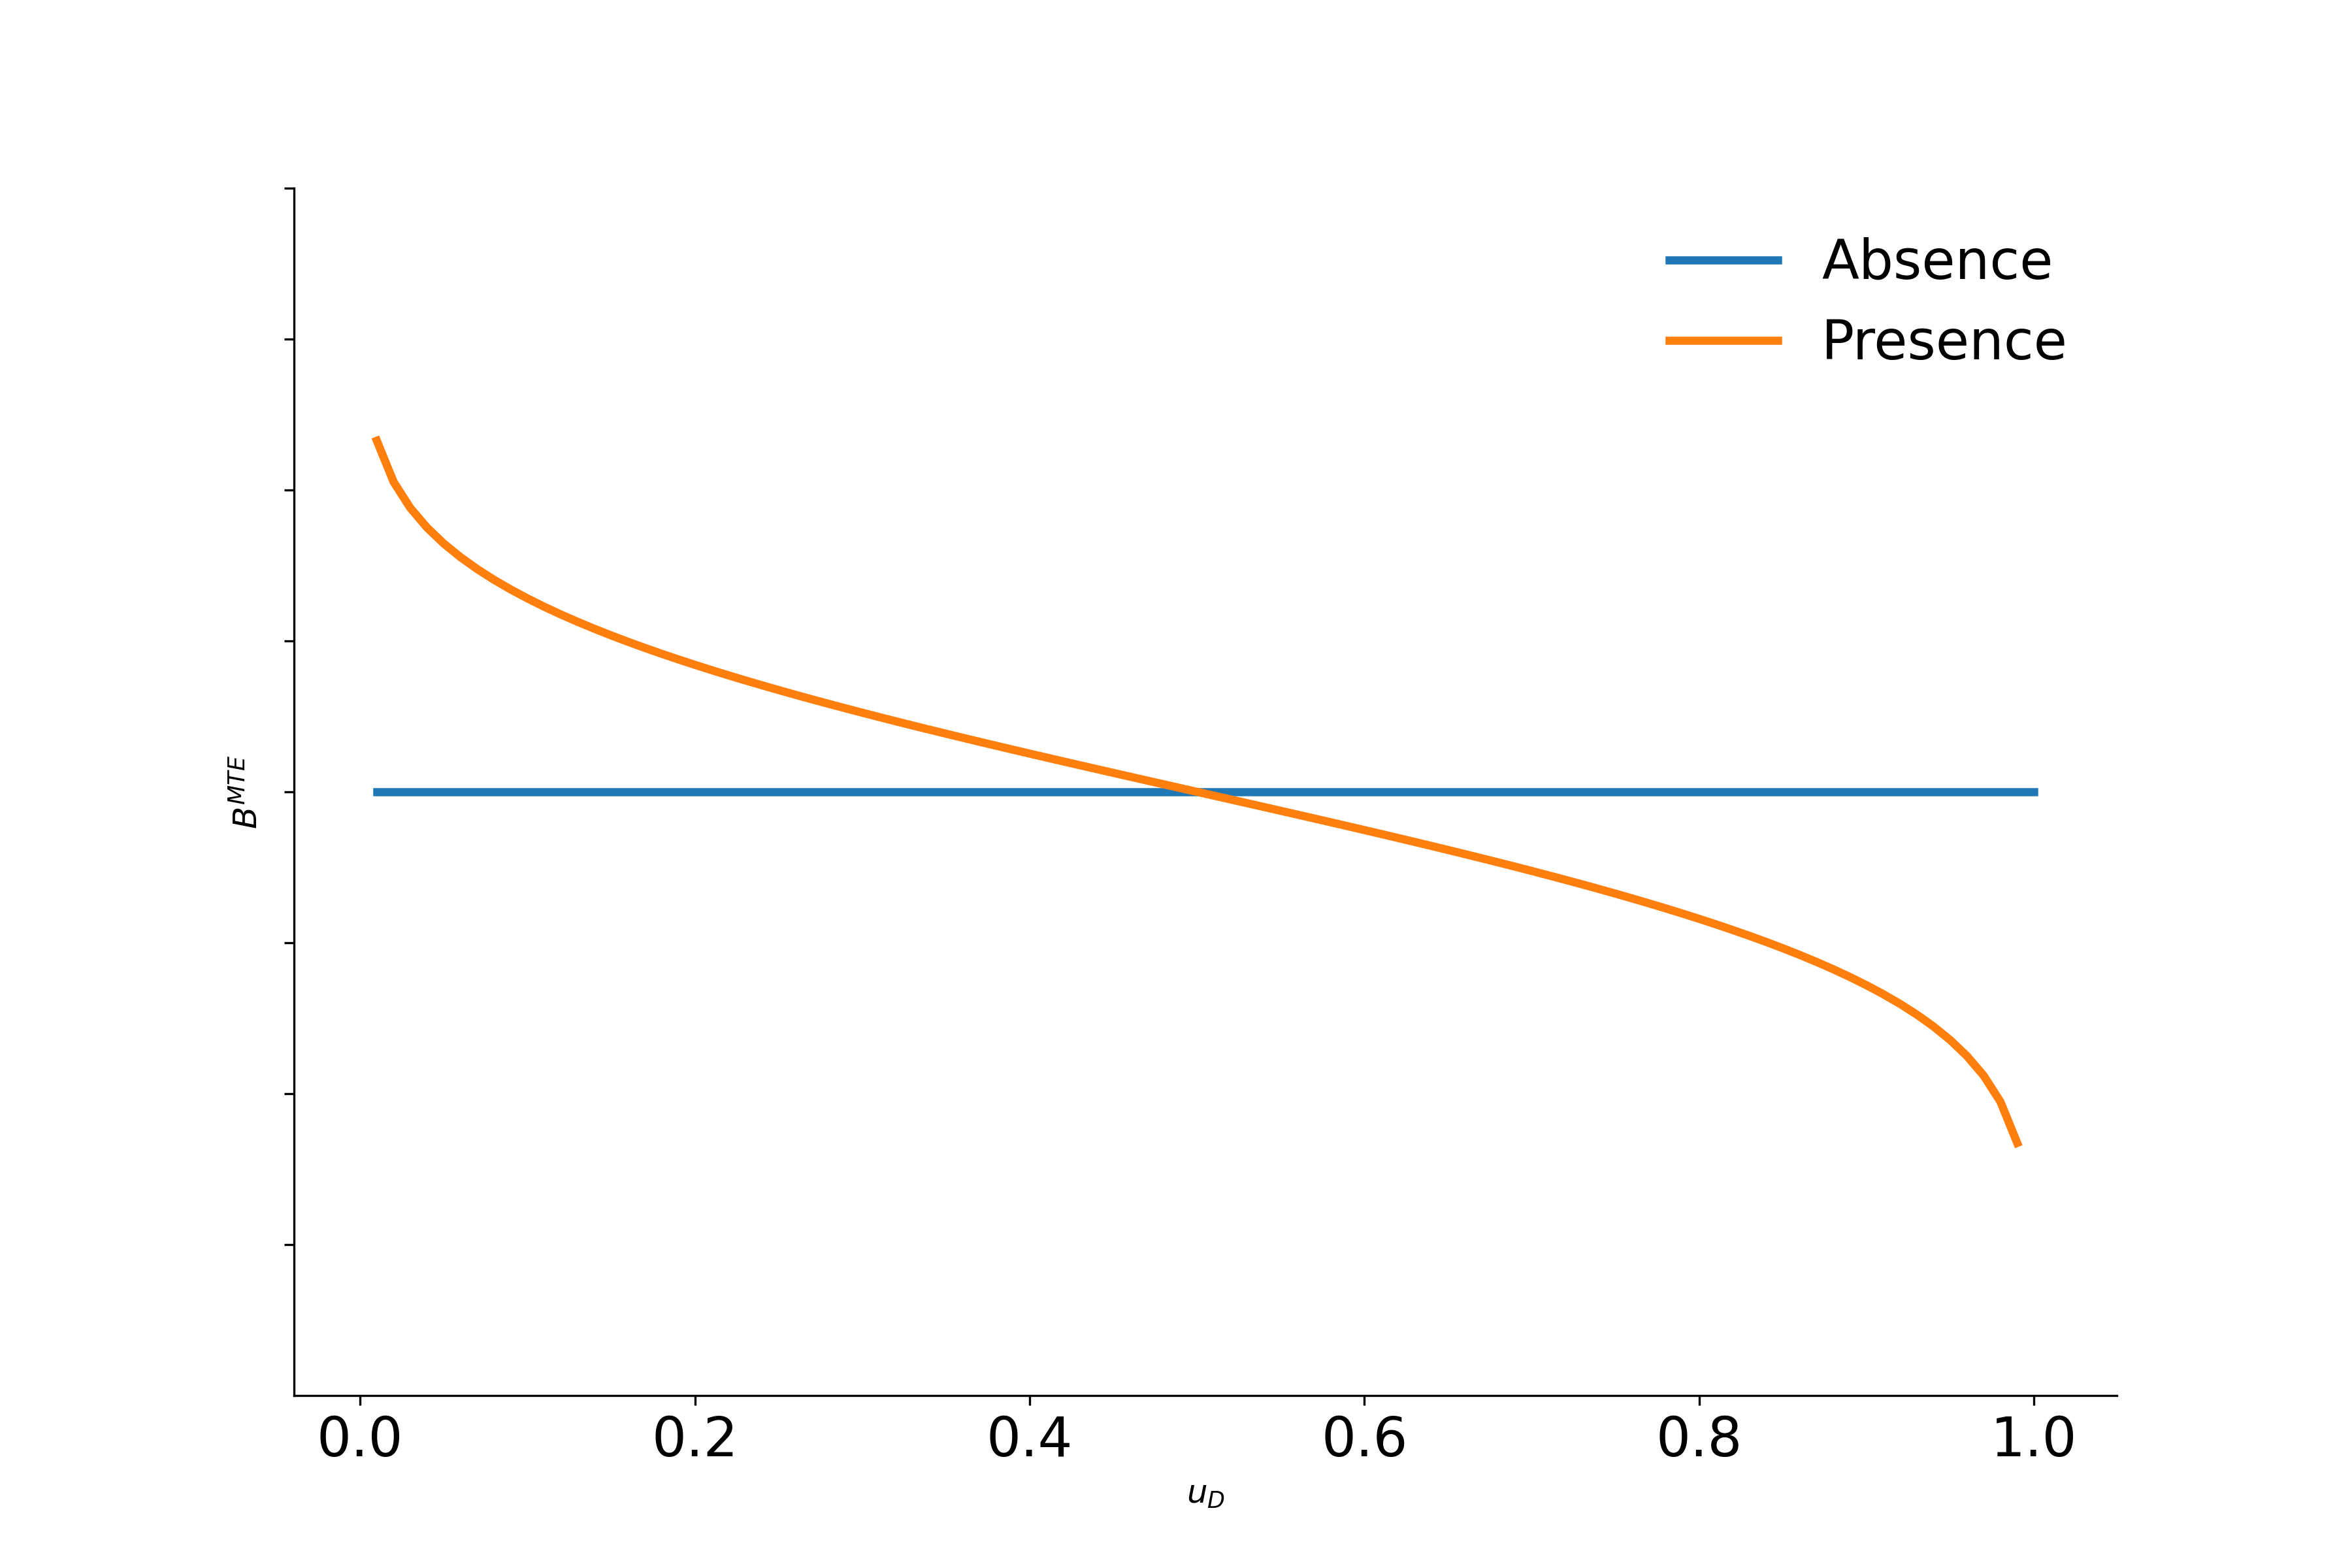
\includegraphics{fig-static-model-marginal-benefit}}
\end{figure}


\end{boenumerate}

\begin{boenumerate}

\item The individual effect of treatment $B$ is defined as the difference in potential outcomes $Y_1 - Y_0$. The unobservable $U$ is the only source of heterogeneity in the model. Given its distribution and the selection equation, about 50\% of individuals will select into treatment. However, only about 25\% have a positive benefit of treatment.

\item The conventional average treatment effects are defined below.
%
\begin{align*}
    B^{ATE} & = E[Y_1 - Y_0 ]\\
    B^{TT}  & = E[Y_1 - Y_0 \mid D = 1]\\
    B^{TUT} & = E[Y_1 - Y_0 \mid D = 0]
\end{align*}
%
Their policy-relevance is limited, as they correspond to extreme policy alternatives. For example a stylized version of the Affordable Care Act, where health insurance coverage was universal after the implementation of the reform. As a considerable share of Americans was already covered before, this corresponds to the $B^{TT}$. A focus on average effects might mask considerable heterogeneity in benefits.

Figure \ref{Distribution of benefits} shows the distribution of benefits. All individuals with a benefit above -0.25 select into treatment because it still holds that $0.50 > U$.

\begin{figure}[htp]\centering
\caption{Distribution of benefits}\label{Distribution of benefits}
\scalebox{0.5}{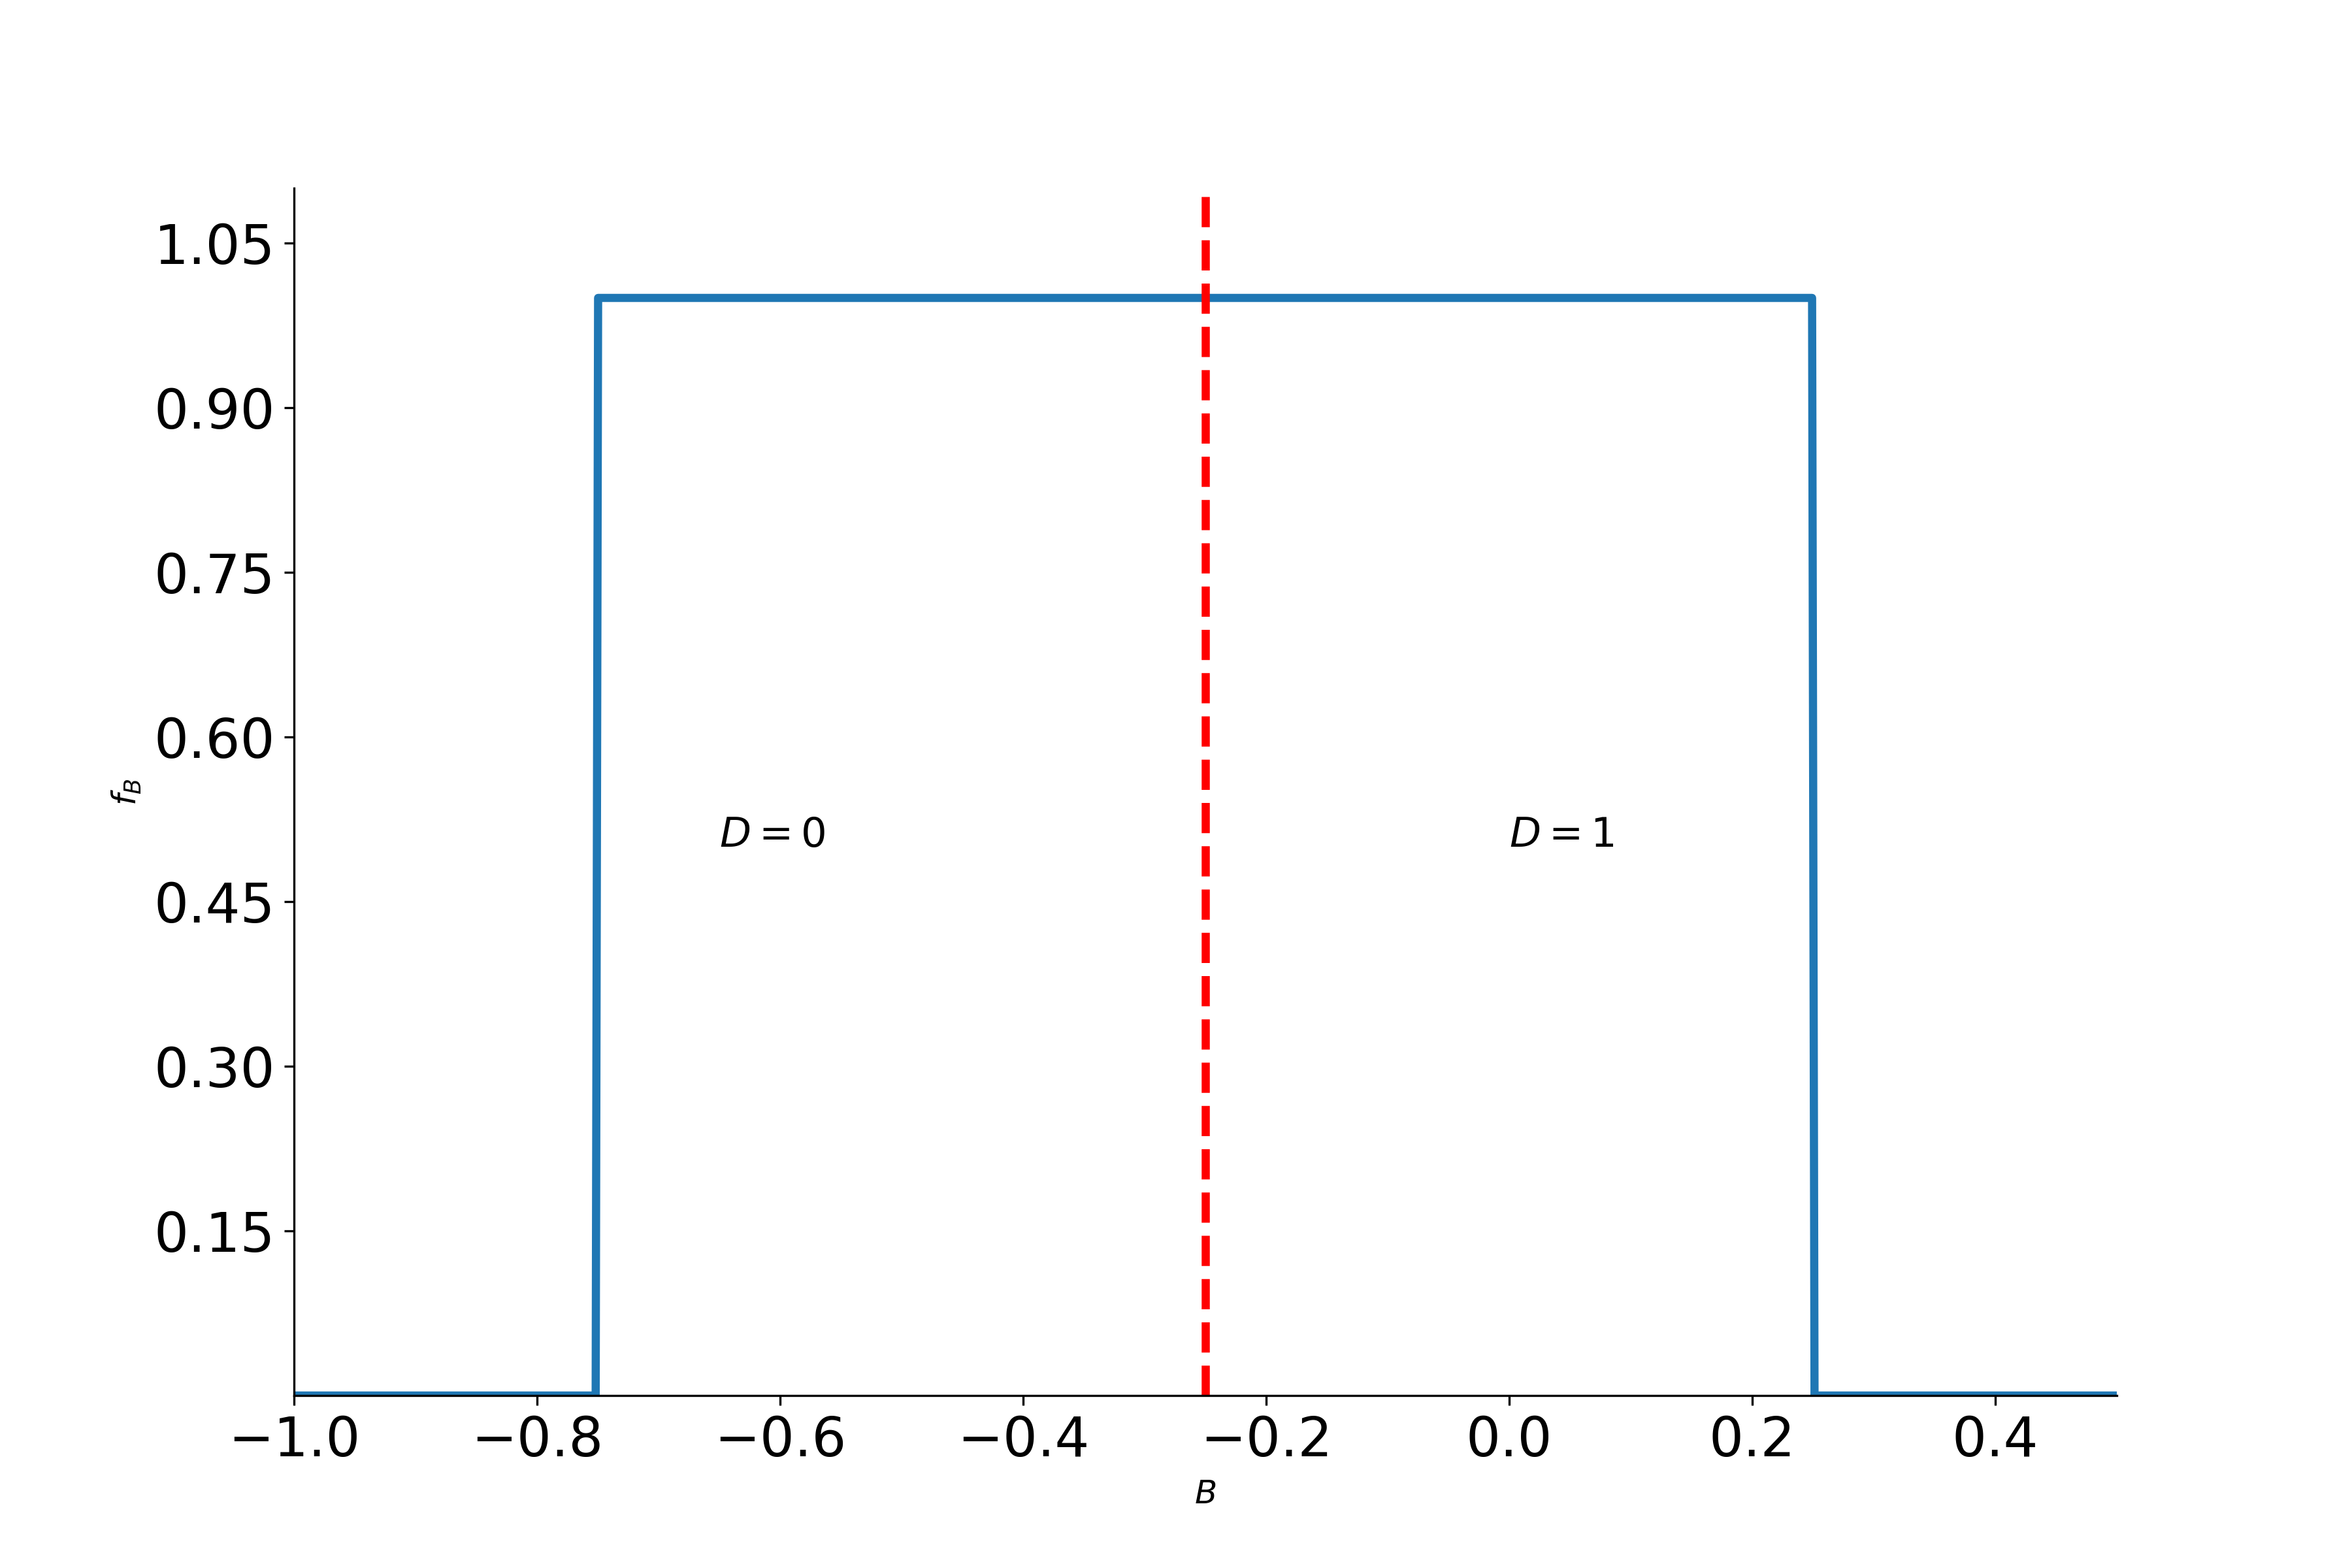
\includegraphics{fig-static-model-distribution-benefits}}
\end{figure}

The conventional effects of treatment are calculated as:
%
\begin{align*}
    B^{ATE} & = -0.25 \\
    B^{TT}  & =  0.00\\
    B^{TUT} & = -0.50
\end{align*}


\item The concept of essential heterogeneity describes the idea that individuals select their treatment status based on unobservable gains from treatment even after conditioning on unobservables. More formally,

\begin{align*}
    Y_1 - Y_0 \notindep D\quad \mid X = x.
\end{align*}

The parameterized model does exhibit essential heterogeneity as individuals with the highest dislike to select into treatment $U$ have the least to gain.


\item The marginal benefit is the average effect of treatment for individuals at different quantiles of the first-stage unobservable $V$. More formally,

\begin{align*}
    B^{MTE}(u_D) = E [Y_1 - Y_0 \mid U_D = u_D].
\end{align*}

Figure \ref{Marginal benefit of treatment} shows the marginal benefit of treatment for the parameterized model.

\begin{figure}[htp]\centering
\caption{Marginal benefit of treatment}\label{Marginal benefit of treatment}
\scalebox{0.50}{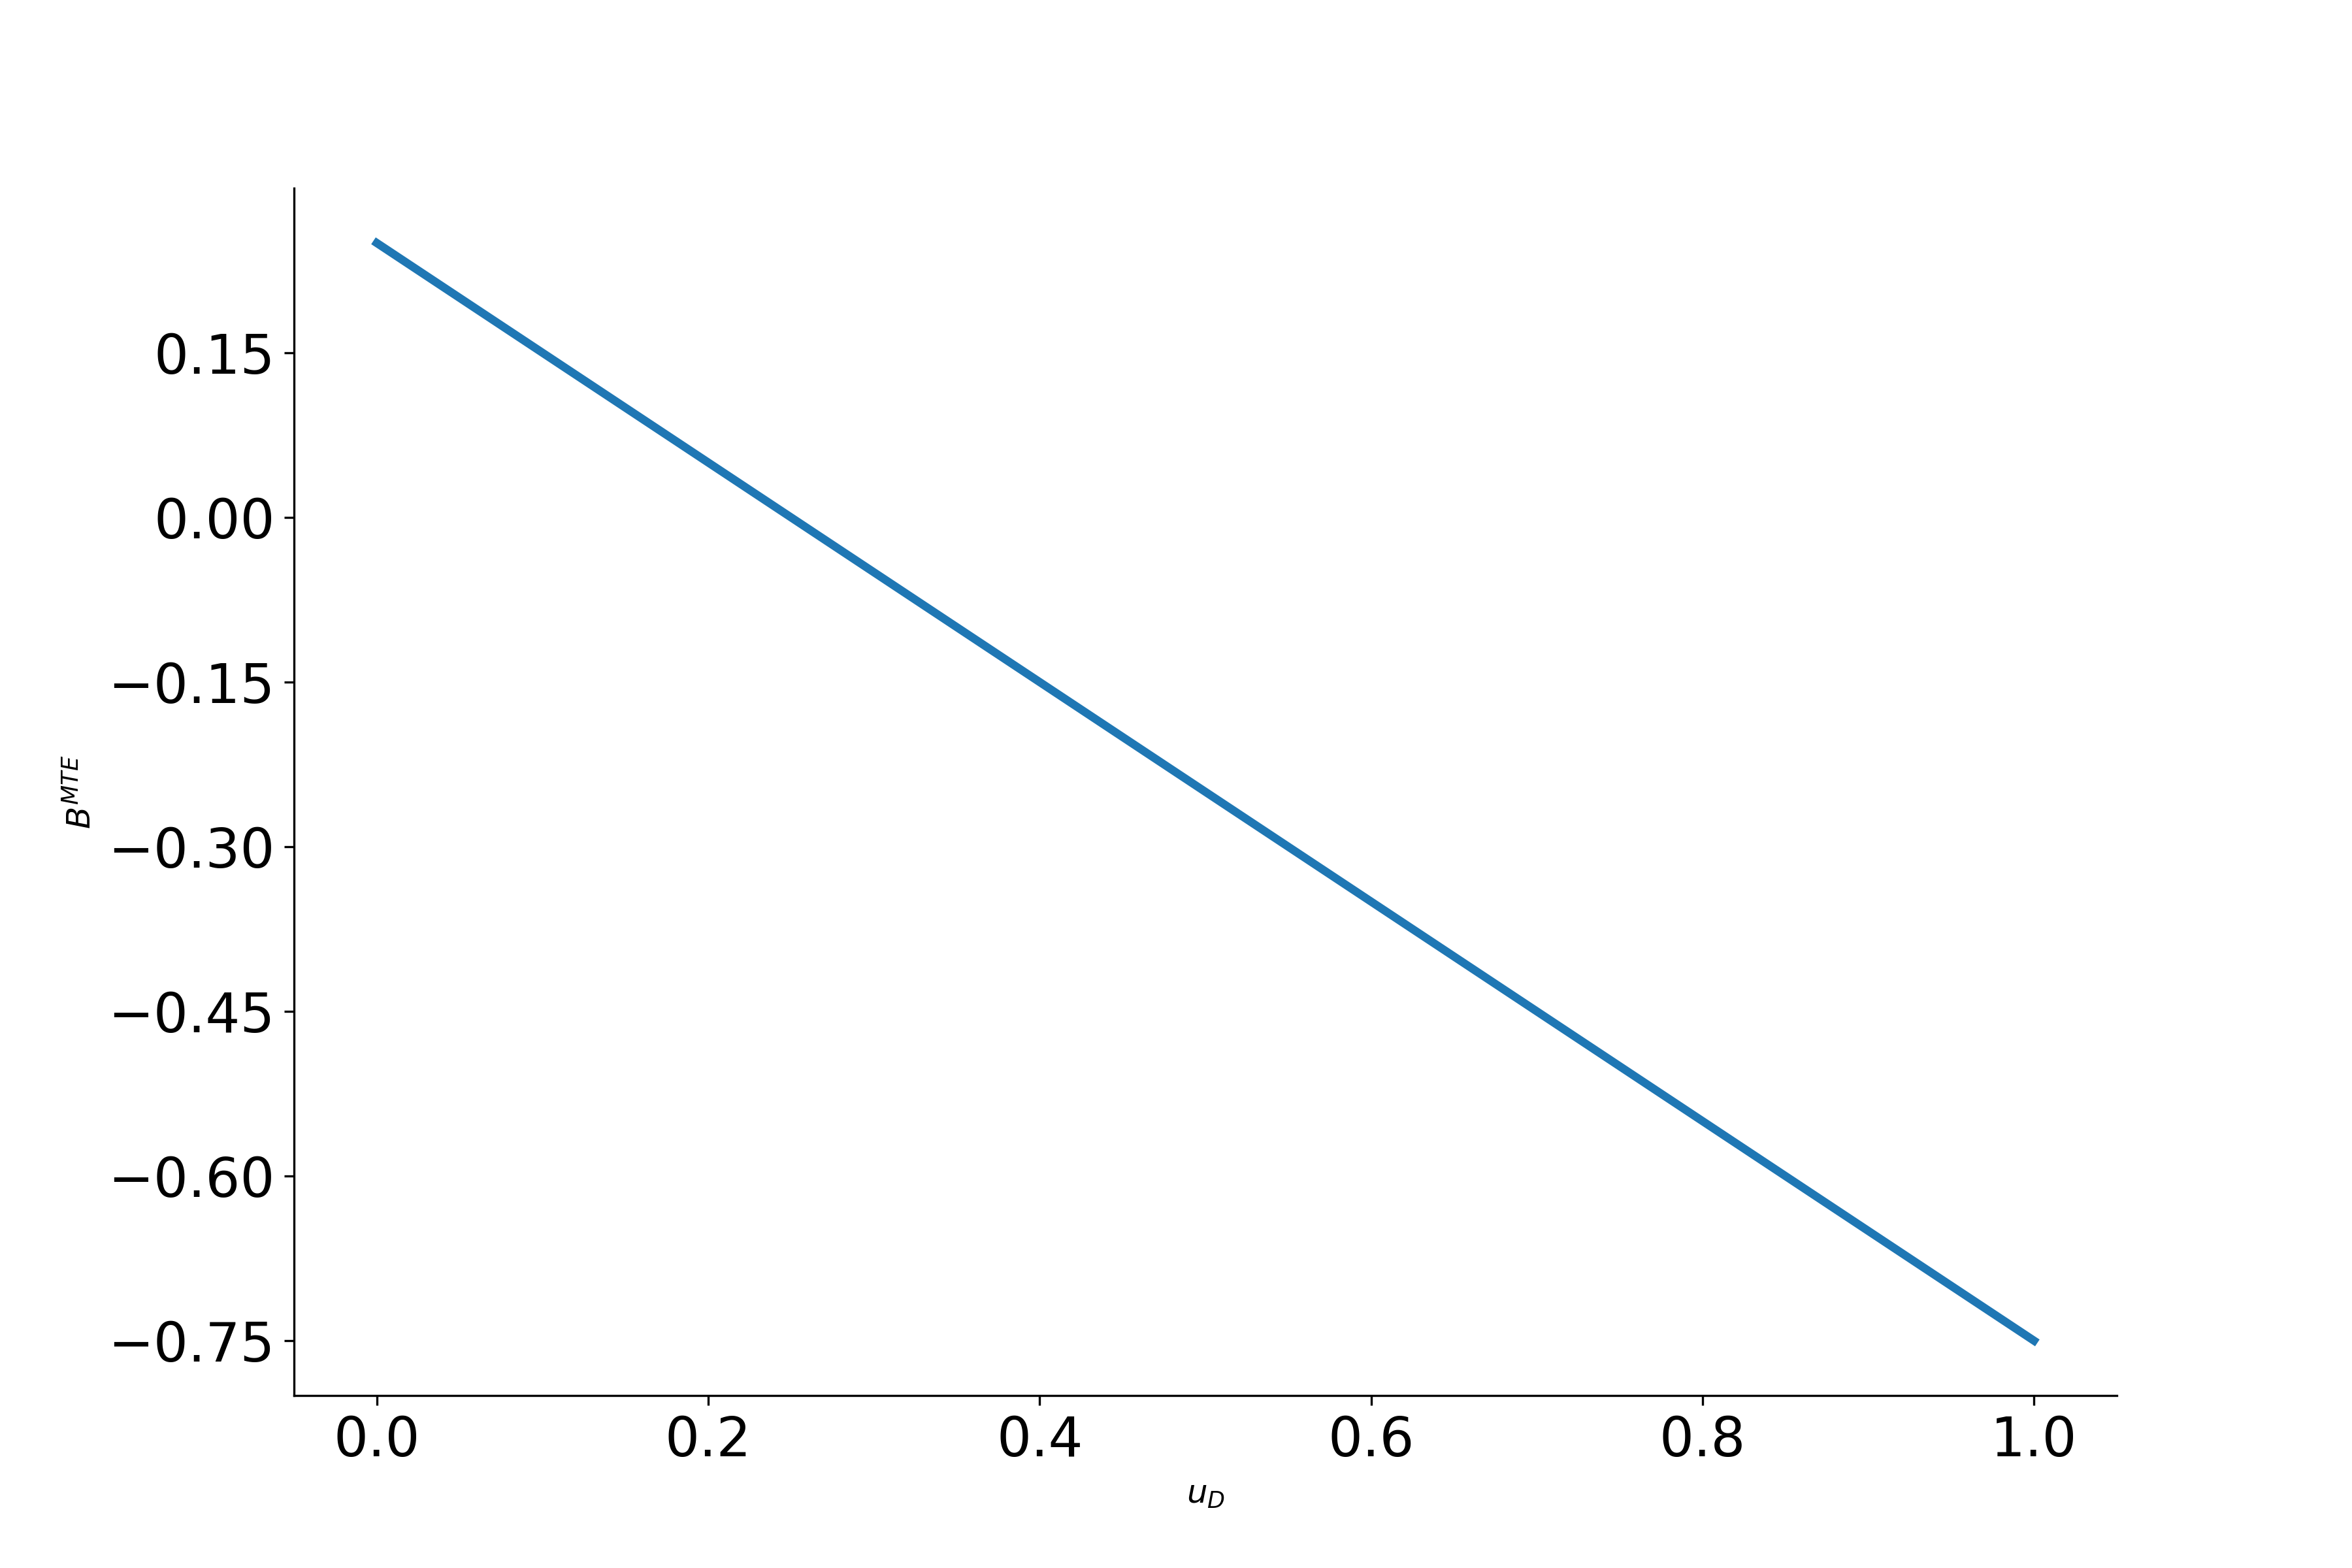
\includegraphics{fig-static-model-marginal-benefit-linear}}
\end{figure}

\end{boenumerate}
%-------------------------------------------------------------------------------
\FloatBarrier\subsection{Dynamic model of educational choice}
%-------------------------------------------------------------------------------
\begin{boenumerate}

\item The Mincer equation is stated below.
%
\begin{align*}
\ln{Y(s, x)} = \alpha + \rho_s s + \beta_0 x + \beta_1 x^2 + \epsilon
\end{align*}
%
The Mincer equation imposes a linear and homogeneous return to schooling and additive separability between schooling and work experience. There is no role for uncertainty and thus no distinction between ex ante and ex post returns. There exist numerous alternative return concepts such as the internal rate of return and the true return.

\begin{itemize}
\item Log-earnings experience profiles are parallel across schooling levels.
\begin{align*}
\frac{\partial \ln{Y(s, x)}}{\partial s \partial x} = 0
\end{align*}
\item Log-earnings age profiles diverge with age across schooling levels.
\begin{align*}
\frac{\partial \ln{Y(s, x)}}{\partial s \partial t} > 0
\end{align*}
\item The variance of earnings over the life cycle has a U-shaped pattern.
\end{itemize}

\item Everybody will go to school for one more year.

\begin{figure}[htp]\centering
\caption{Final schooling level}\label{Final schooling level}
\scalebox{0.5}{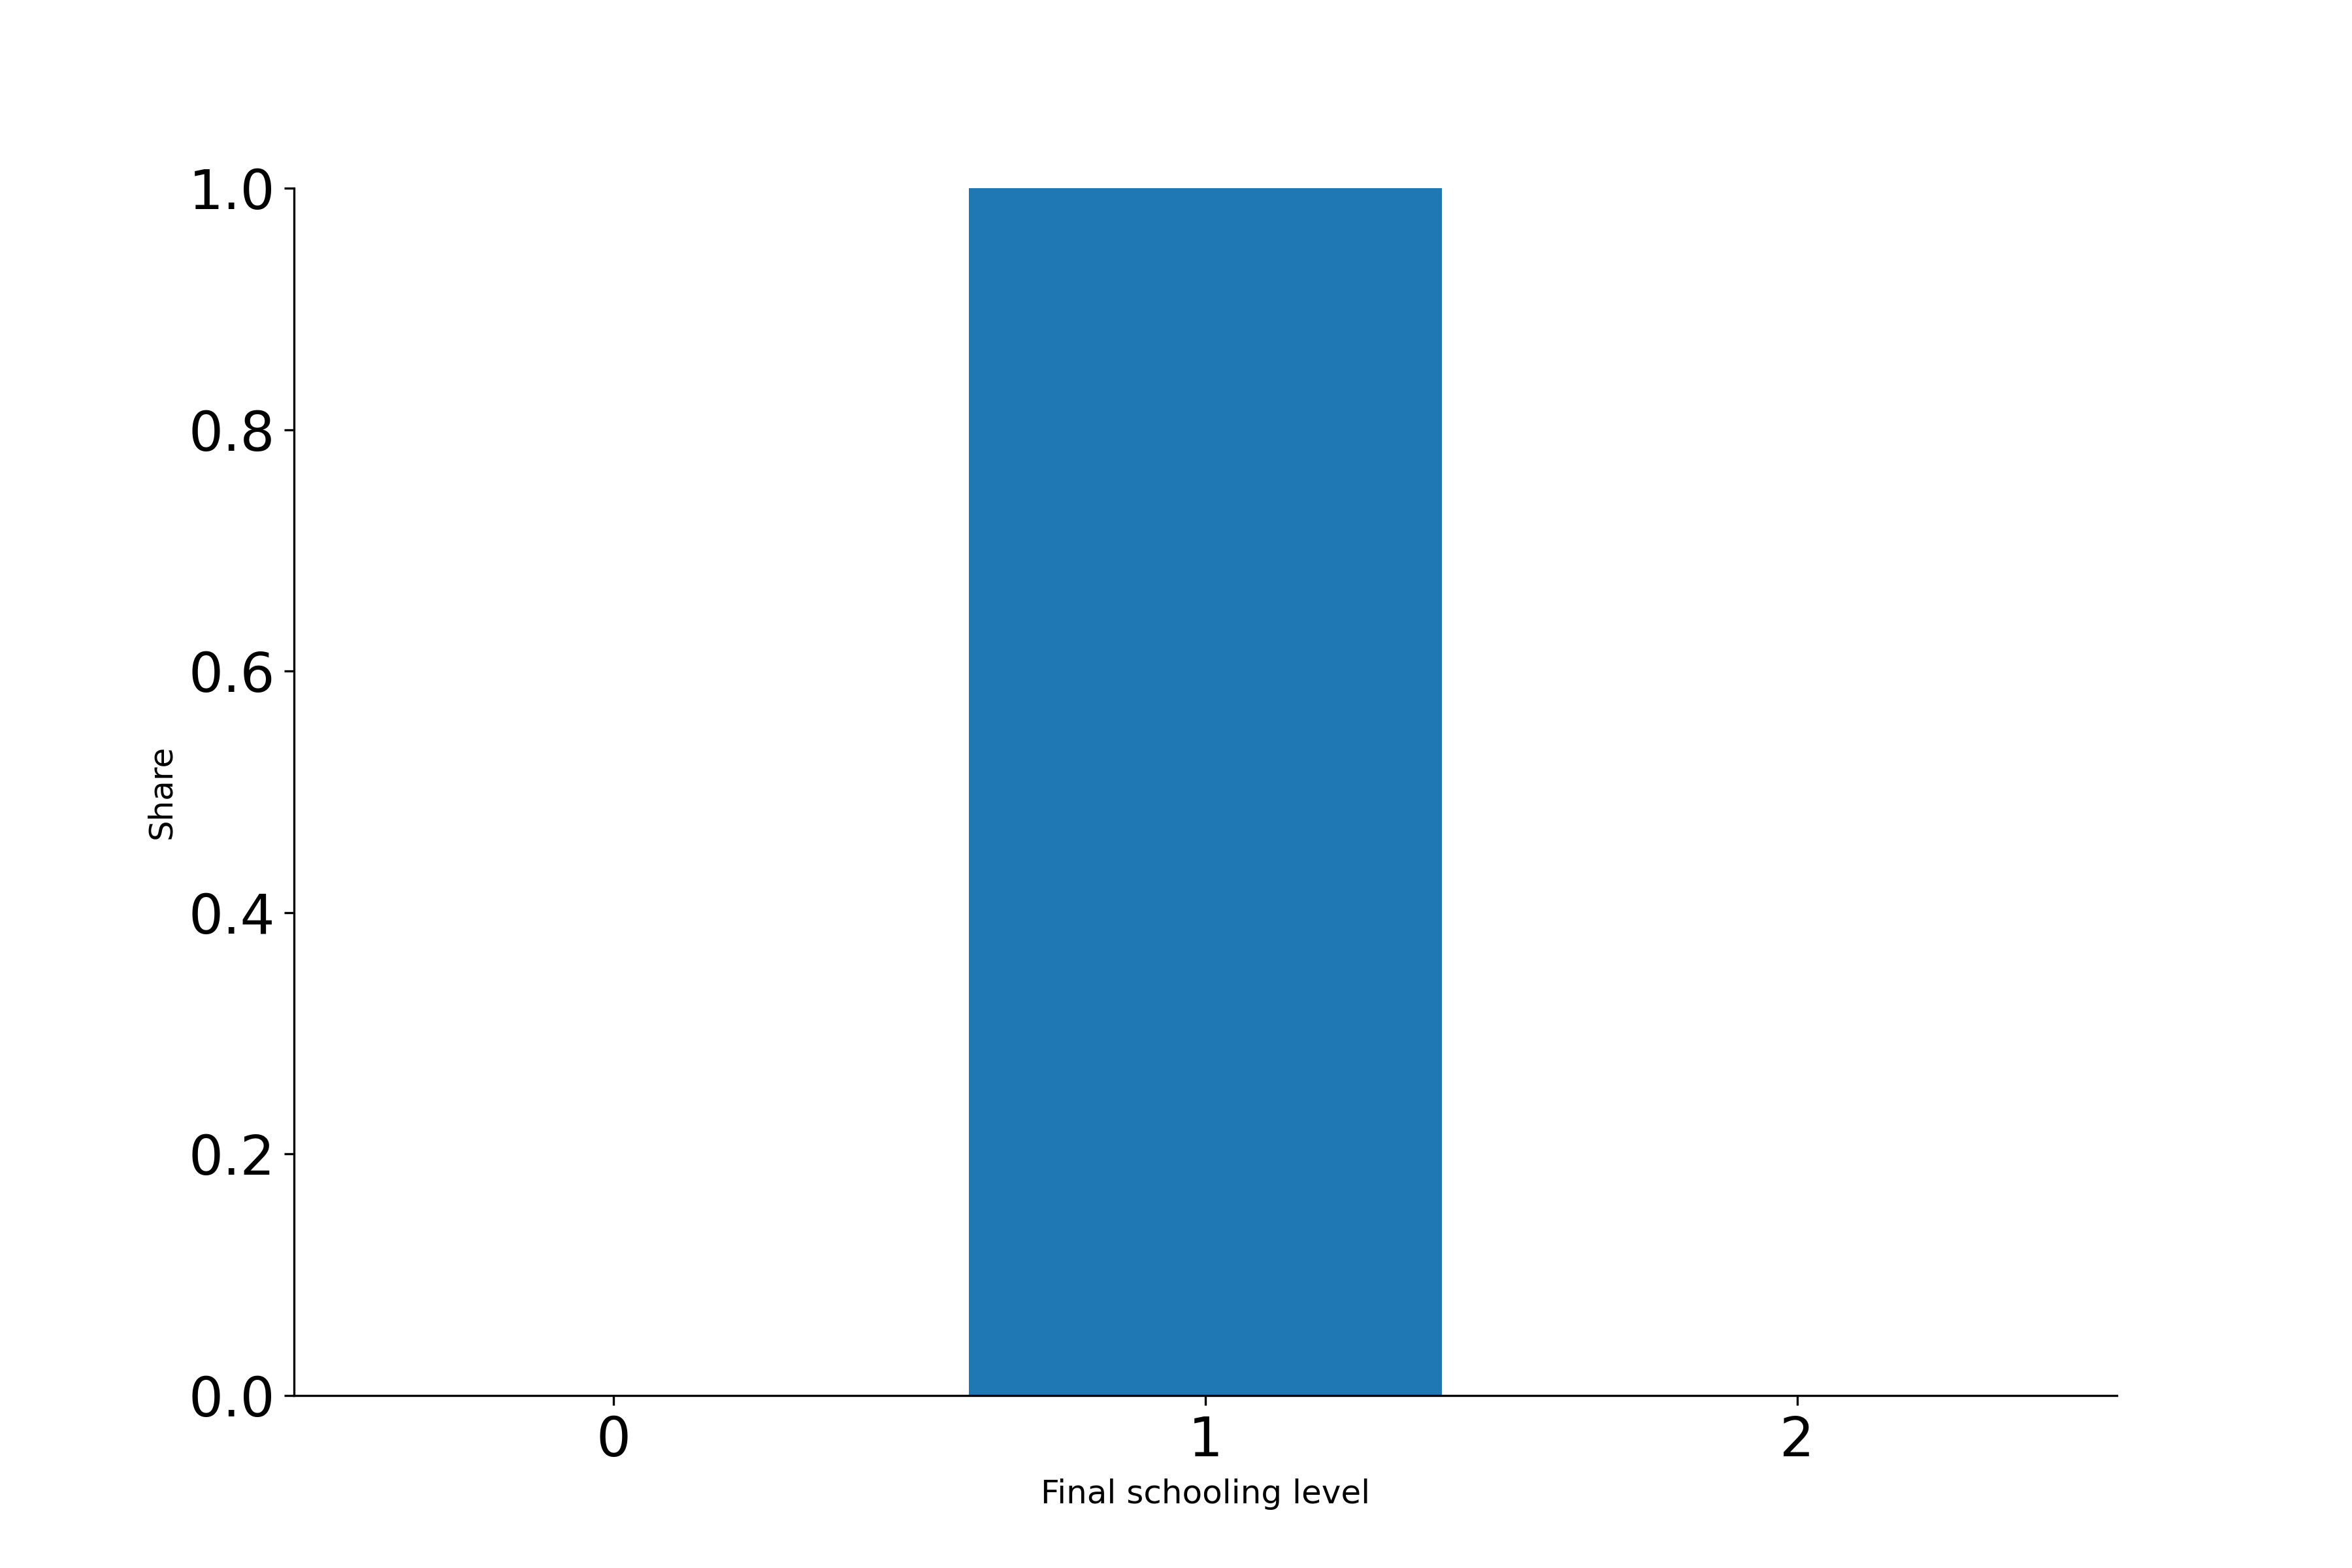
\includegraphics{fig-dynamic-model-final-schooling}}
\end{figure}

\item The value and true return are defined below.

\begin{align*}
V_s & = \max\left\{Y_s, E_s(V_{s+1})\right\}\\
R_{s, s - 1} & = \frac{\E_{s - 1}\left[V_s\right] - Y_{s - 1}}{Y_{s -1}}
\end{align*}

The value of zero schooling is $V_0 = 2$ and the true return amounts to $R_{1, 0} = 3$

\item The option value is defined below.
%
\begin{align*}
O_{s, s - 1} = \E_{s - 1}\left[V_s - Y_s\right]
\end{align*}
%
The option value captures the possibilities to continue schooling even further after completing a schooling level. Given the model parameterization, the option value amounts is zero.
\end{boenumerate}
